\documentclass{article}

% PACKAGES
\usepackage[english]{babel}
\usepackage[letterpaper,top=2cm,bottom=2cm,left=3cm,right=3cm,marginparwidth=1.75cm]{geometry}
\usepackage{amsmath,amssymb}
\usepackage{graphicx}
\usepackage[colorlinks=true, allcolors=blue]{hyperref}
% Dani packages
\usepackage{xcolor}
\usepackage{xspace}
%\newcommand{\note}[1]{{\color{red} \textbf{#1}}}
\DeclareRobustCommand{\dm}[1]{{\color{blue}(\textbf{Dani}: \textit{#1}\xspace)}}
% averaging brackets
\DeclareRobustCommand{\lla}{\left\langle}
\DeclareRobustCommand{\rra}{\right\rangle}
% Flow parameters
\DeclareRobustCommand{\Reynolds}{\ensuremath{R\hspace{-0.1em}e}\xspace}     % bulk Reynolds
\DeclareRobustCommand{\Womersley}{\ensuremath{W\hspace{-0.25em}o}\xspace}    % Womersley number
\DeclareRobustCommand{\Amplitude}{\ensuremath{A}\xspace}    % Amplitude

% Title
\title{CHAPTER 9: Model for puffs and slugs in pulsatile pipe flow}
\date{}
%%%%%%%%%%%%%%%%%%%%%%%%%%%%%%%%%%%%%%%%%%%%%%%%%%%%%%%%%%%%%%%%%%%%%%%%%%%%%%%%%%%%%%%%%%%%%%%%
% BEGIN DOCUMENT
%%%%%%%%%%%%%%%%%%%%%%%%%%%%%%%%%%%%%%%%%%%%%%%%%%%%%%%%%%%%%%%%%%%%%%%%%%%%%%%%%%%%%%%%%%%%%%%%
\begin{document}
\maketitle
%%%%%%%%%%%%%%%%%%%%%%%%%%%%%%%%%%%%%%%%%%%%%%%%%%%%%%%%%%%%%%%%%%
% Introduction: 
% - Motivation to develop an extension of the model: 
%   · We observe puffs and slugs in pulsatile pipe flow...
%   · Pulsatile pipe flow influenced by many features...
% - We first explain the extension of the model 
% - We show some results of the model, compared with DNS, justify model decisions
% - We talk about limitations and future prospects
Turbulence in pulsatile pipe flow first appears in the form of localized turbulent patches. These patches are similar to the puffs and slugs observed in steady pipe flow \dm{Esta informacion estara en otros capitulos, secciones. Citalos aqui.}. Depending on the flow parameters, puffs and slugs show different behaviours. At low $Wo \lesssim 4$ they behave quasisteadily and are solely affected by the instantaneous Reynolds number $Re_{i}= U\left( t \right) Re$. When $Re_{i} \lesssim 2000$ they tend to quickly decay, whereas when $Re_{i} \gtrsim 2300$ they tend to elongate and grow in magnitude. At high pulsation frequencies $Wo \gtrsim 20$ they are unaffected by the pulsation and depend only on the mean $Re$, as in steady pipe flow \dm{Cita Xu Avila 2017 2018}. In the intermediate regime $5 \lesssim Wo \lesssim 17$ puffs are modulated by the pulsation. In this intermediate regime, the front speed and survival of puffs depends on the combination of $Re$, $Wo$ and $A$. Moreover at these pulsation frequencies, and at $A\gtrsim 0.5$ our results suggest that puffs take advantage of the instantanous linear instability of the laminar profile to survive \dm{Cita Entropy, capitulos, secciones y eventualmente un paper del modelo de Barkley}.

In this chapter we adapt the BM of steady pipe flow \dm{Cita el capitulo o sección} to pulsatile pipe flow at $Wo \geq 4$. At lower $Wo$ puffs behave quasi-steadily, and we understand that there is no need to model their behaviour. The motivation to develop a simple model for puffs and slugs in pulsatile pipe flow is two-fold.

On the one hand, we would like to have a tool that, in an efficient way, can perform simulations of turbulence in a huge parameteric regime of pulsatile pipe flow. We have mentioned how the behaviour of puffs and slugs can dramatically change, when changing one of the flow parameters. A simple model could approximate the puffs survival or front speed changes when changing the parameters in a fast way. It could be eventually used to develop control laws of puffs and slugs in pulsatile pipe flow.

On the other hand, a simple model could help us understand the dynamics behind puffs and slugs in pulsatile pipe flow. At either very low or very large frequencies the behaviour of puffs and slugs are almost identical to the case of steady pipe flow. In the former, puffs and slugs adjust to the instantaneous mean shear, while on the latter to the time averaged mean shear. As seen in \dm{Citar capitulo (seccion) del modelo de Barkley}, in the case of steady pipe flow, the dynamics of puffs and slugs are mainly determined by the non-linear interaction between the mean shear and the turbulence intensity. Thus it is safe to assume that slight changes to the original BM, that include the changes on the mean shear due to the pulsation, can approximate well the behaviours of puffs and slugs in these frequencie regimes. At intermediate frequencies the behaviour of puffs and slugs is more complex. They are elongated and modulated by the pulsation, and, according to our results, they make use of other dynamics, apart from the state of the mean shear, to survive. It is thus worth it to try modify the model, and study which dynamics should be included in order to model puffs at these frequencies. 

The rest of the chapter is organized as follows. First we describe our proposed changes and extensions to the original model of Barkley, to adapt it to pulsatile pipe flow. We provide some justification to the changes, together with examples of other design options. Second, we present the results of the extended Barkley model (EBM) alone and compared with results of individual DNS of pulsatile pipe flow. We finally comment on the limitations of the model. 



%%%%%%%%%%%%%%%%%%%%%%%%%%%%%%%%%%%%%%%%%%%%%%%%%%%%%%%%%
% Section: the model
% - Phylosophy
% - We justify the changes... (include maybe results without those changes?)
% - We follow the description of the BM in chap 5
\section{Extension to the BM for pulsatile pipe flow}
In this section we describe the modifications we propose in order to extend the BM to pulsatile pipe flow. The core idea of the extended Barkley model (EBM) is the same idea behind the original BM: the non-linear interaction between the turbulence intensity $q$ and the mean shear $u$. As in the BM, in the EBM $u$ corresponds to the centerline velocity, as a proxy to the  mean shear. The instantaneous laminar profile of pulsatile pipe flow can be much complex than a simple parabolic profile \dm{Aqui quizas sería interesante citar un posible apendice donde incluya un catalogo de perfiles laminares de flujos pulsatiles, una ristra de plots parecidos a la figura 4 del paper de waveforms. En el caso del paper podría citar algun paper (el de Womersley?)}, and therefore the shape of the shear can not be described by a single parameter like in steady pipe flow. We here assume that at relatively small pulsation amplitudes $A \lesssim 0.5$, the centerline velocity still represents a good approximation to the state of the mean shear. We further assume that the state of the mean shear at higher amplitudes $A \gtrsim 0.5$, can be approximated with a parameter inspired by the physics of pulsatile pipe flow, without the need of an additional model variable. 

Our modifications have a constraint and fulfil a requireement. The EBM is constrained to pulsatile pipe flows with $\bar{U}\left( t \right) \geq 0$. As we show below the resultant EBM returns to the original BM when either $Wo=0$ or $A=0$. As we did in \dm{chapter 5, (section ?)} with the BM, in the rest of the chapter we describe the EBM from its local to its spatially extended dynamics.





% Local dynamics of the mean shear:
% - First the time dependence... \bar{U}(t), Uc(t)
% - Second the effect of pressure gradient and viscosity (By equilibrium of forces...)-> validate with Laminar calculations!
\subsection{Local dynamics of the mean shear}
In pulsatile pipe flow, the laminar centerline velocity $U_{c} \left(t \right)$ and bulk velocity $\bar{U} \left( t \right)$ are functions of time. While the bulk velocity is set by the pulsation, the evolution of $U_{c}\left( t \right)$ can be obtained from the NSE. First we assume laminar pipe flow, $\pmb{u}\left(r,\theta,x,t\right)\rightarrow\left(0,0,U\left(r,t\right) \right)$:
\begin{align}
\frac{\partial U}{\partial t}= Gp\left(t\right) + F_{visc}\left(r,t\right) \text{,}
\end{align}
and secondly we set $r \rightarrow 0$. Here,
\begin{align}
Gp\left(t\right)=- \frac{\mathrm{d} P}{\mathrm{d} x} \left(t \right) \text{,}
\end{align}
is the pressure gradient that drives the flow at the desired $\bar{U} \left( t \right)$, and:
\begin{align}
F_{visc}\left(r,t\right)= \frac{1}{Re} \left( \frac{\partial^{2}U}{\partial r^{2}} + \frac{1}{r} \frac{\partial U}{\partial r} \right) \text{.}
\end{align}
When $r \rightarrow 0$,
\begin{align}
F_{v_{0}} \left(t \right)=\lim_{r \to 0} F_{visc} = \lim_{r \to 0} \left[ \frac{1}{Re} \left( \frac{\partial^{2}U}{\partial r^{2}} + \frac{1}{r} \frac{\partial U}{\partial r} \right) \right] \text{.}
\label{eq:limFvisc}
\end{align}
If one applies L'Hopital's rule to the limit in equation~\ref{eq:limFvisc},
\begin{align}
F_{v_{0}} =  \frac{2}{Re} \frac{\partial^{2}U}{\partial r^{2}} \text{,}
\end{align}
and, for $U_{c}\left(t\right)=U\left(t,r=0\right)$,
\begin{align}
\frac{\partial U_{c}}{\partial t}=Gp\left(t\right) + F_{v_{0}}\left(t\right) \text{.}
\label{eq:centerline}
\end{align}
Note that the time average of the right hand side of equation~\ref{eq:centerline} yields $\left \langle Gp\left(t\right) + F_{v_{0}}\left(t\right) \right \rangle=0$

The equilibrium of forces described in equation~\ref{eq:centerline} must be included in the model since, when the flow is locally laminar $\left(q=0\right)$, $u\equiv U_{c}$. Thus the original equation \dm{Citar la ecuacion locu del capitulo 5 de la tesis, en el caso del paper de la seccion correspondiente}, is extended to:
\begin{align}
\dot{u}=g_{EBM}\left(q,u\right)= \epsilon_{1} \left(U_{c}\left(t\right)-u \right) + \epsilon_{2} \left(\bar{U}\left(t\right)-u \right)q + Gp\left(t\right) + F_{v_{0}}\left(t\right) \text{,}
\label{eq:loc_u_EBM}
\end{align}
where $U_{c}$, $G_{p}$ and $F_{v_{0}}$ are the corresponding laminar centerline velocity, pressure gradient and the viscous force at the center of the pipe. They can be precomputed by numerically integrating equation~\ref{eq:centerline}.

 





% Local dynamics of turbulence intensity
% - First the time dependence: r!, U_c...
% - Second the effect of the inflection point
% - We opt for directly the inflection point ...
\subsection{Local dynamics of turbulence intensity}
In the original BM, the control parameter $r$ sets the production of turbulence intensity. As we observe in our DNS \dm{Aqui puedes citar el paper de Entropy (en el caso del paper), o incluso resultados que puedes incluir de nueva cosecha en el paper(tengo calculada la produccion en cada posicion axial y phase averaged!). En el caso de la tesis cita resultados de probablemente el capitulo 7.} turbulent production is modulated by the pulsation. We model this feature by considering a time dependant $r_{EBM}\left( t \right)= r \left( Re \right) \cdot \bar{U}\left(t+\phi\right)$, where $r$ is constant, and it is calculated using the mean Reynolds $Re$, and $\bar{U}\left(t + \phi\right)$ is a time shifted bulk velocity. In our DNS we observe a time delay between the maximum integrated turbulence intensity $\left \langle q \right \rangle_{r,\theta,z}$ and the bulk velocity $\bar{U}$ \dm{Aquí añade una figura que demuestre esto. Quizas puedas coger todas las DNS y generar un plot donde se vea (a Re constante?) como cambia "phi" con Wo. Tambien puedes referenciar otro capitulo (seccion en el paper)}. We find that the phase lag $\phi \left(Wo\right)$ between the pressure gradient and laminar profile that it generates, first derived by Womersley \dm{Cita Womersley}, is a good approximation. Moreover, the phase lag is a sole function of the Womersley number, and it has an analytical expresion.

As we show in \dm{Aqui deberas citar el capitulo 7 y 8, y la seccion correspondiente del paper, donde hables del inflection point y de sus effectos en las DNS}, at certain $5 \lesssim Wo \lesssim 17$ and $A\gtrsim 0.5$, the laminar profile of pulsatile pipe flow is very different to the parabolic profile of the steady case \dm{En el caso de la tesis citar el apendice con el catalogo de perfiles laminares}, and can even be instantaneously unstable. \dm{Citar capitulo 6, paper de waveforms en el paper.} The centerline velocity $u$ alone is not able to capture this features of the mean shear. Since in this case we have decided not to add any new variable to the model, the effect of the instantaneous shape and effects of the mean shear are modeled by adding to the local dynamics of $q$ in equation \dm{Cita la ecuacion locq en el capitulo q} the term $+ \gamma \lambda \left(t\right) q$. Here $\lambda \left(t\right)$ represents how linearly unstable the laminar profile is due to the presence of inflection points, and it is always $\lambda\geq 0$. It corresponds to the maximum eigenvalue of the instantaneous laminar profile, as we computed it in \dm{Cita el capitulo donde hables de la estabilidad lineal instantanea y el catalogo final de flujos pulsatiles con su lambda, y en el caso del paper cita el de waveforms y añade: We compute the eigenvalues of the laminar profile at certain time steps as if the profile was instantaneously steady. We then assume that the maximum eigenvalue is continuous in time and construct $\lambda \left(t \right)$}. The parameter $\gamma$ models the effect $\lambda$ has on the growth of $q$. It represents the accuracy of the quasi-steady assumption used to compute $\lambda$. In theory it should scale with the length of the period in terms of flow units $T=\frac{\pi Re}{2 Wo^{2}}$. The idea is that, the longer the period is, the slower the mean shear evolves with respect to the turbulent structures. We find a good compromise with:
\begin{align}
\gamma = 0.23 \log \left(T\right) \text{.}
\label{eq:gamma_EBM}
\end{align}

By introducing these changes to the model, the local dynamics of $q$ in the EBM are described by the following ODE:
\begin{align}
\dot{q}=f_{EBM}\left(q,u\right)=q \left[r\bar{U}\left(t+\phi\right)+\gamma \lambda + u-U_{c}\left(t\right)-\left(r\bar{U}\left(t+\phi\right)+\delta \right) \left(q -1 \right)^{2} \right]\text{.}
\label{eq:loc_q_EBM}
\end{align}



% Spatially extended model: 
% - just comment on the advection term of q...
% - Talk about the importance of the noise term. How do we scale it with Re...
\subsection{Spatially extended and stochastic model}
As for the original BM, the local dynamics alone are not able to describe the behavior of localized turbulence in pulsatile pipe flow. One needs to also consider advection, diffusion and stochstic effects. In the case of the centerline velocity the spatially extended equation is equal to equation \dm{Cita Capitulo 5 eqPDEu}:
\begin{align}
\frac{\partial u}{\partial t}=-u\frac{\partial u}{\partial x} + g_{EBM}\left(q,u \right) + \frac{2}{Re}\frac{\partial^{2} u}{\partial x^{2}} \text{.}
\label{eq:PDE_u_EBM}
\end{align}

In the original BM \dm{CITA Cap 5} the velocity at which $q$ is advected is equal to $u-\eta$ where $\eta$ acts as a correction parameter. In the case of pulsatile pipe flow, the advection velocity should also depend on the pulsation. We model this by correcting the velocity by $u-\eta \bar{U}$ instead of simply $u-\eta$:
\begin{align}
\frac{\partial q}{\partial t}=-\left(u-\eta \bar{U} \right)\frac{\partial q}{\partial x} + f_{EBM}\left(q,u \right) + D\frac{\partial^{2} q}{\partial x^{2}} + \sigma \left(Re \right) \tau \left(t,x\right) q \text{,}
\label{eq:SPDE_q_EBM}
\end{align}
Note that, in the EBM $\sigma$ depends on the $Re$. While fitting the model to our DNS results, we noticed how, at certain parameters the magnitude of the noise was critical in order to validate the front speed and lifetimes of the puffs. Wo found that a noise intensity that scales linearly with $Re$, with an upper bound of $\sigma \leq 0.9$:
\begin{align}
\sigma= \left\{\begin{matrix}
0.1 & if & Re \leq 2020\\ 
\frac{3}{5}\cdot \frac{\left(Re-1933 \right )}{1000} & if & 2020<Re<2640\\ 
 0.85 & if & Re\geq 2640
\end{matrix}\right.
\label{eq:sigma_EBM}
\end{align}
produces much better results than a constant value. There are different reasons why the noise amplitude might need to be adjusted to  $Re$, \dm{CITA la ultima seccion de este capítulo}. The most obvious one is that, for increasing $Re$ one expects an increase in the chaotic characteristics of the flow that are modeled with the noise term. However at any sufficiently high $Re$ there should be some chaotic dynamics, therefore the upper bound, and the stochastic term cannot become bigger than the main dynamics of the model, therefore the upper limit. 


\subsection{Overview of the model}
Equations \ref{eq:SPDE_q_EBM} and \ref{eq:PDE_u_EBM} together with the local dynamics \ref{eq:loc_q_EBM} and \ref{eq:loc_u_EBM} and the parameters defined in equations \ref{eq:gamma_EBM} and \ref{eq:sigma_EBM}, define the EBM. Let us highlight three important features of the model.

First, when $A=0$ or $Wo=0$ one recovers the original BM. At $A=0$ or $Wo=0$, there is no oscillatory component in $\bar{U}$ or $U_{c}$, $G_{p}+F_{v_{0}}=0$ and at these $A$ and $Wo$ $\lambda \equiv 0$. 

Second, the control parameter $r$ of the original BM set the behaviour of the localized turbulent patches. In the case of the EBM, the equivalent parameter $r_{EBM}=r \bar{U} \left(t + \phi \right)$ now oscillates between a minima and a maxima, at a frequency set by the combination of $Re$ and $Wo$. As we show below, at low frequencies $Wo \lesssim 4$ we see a quasi-steady behaviour of the puffs. When the instantaneous parameter $r_{EBM} <0$ puffs tend to shrink and decay, whereas at $r_{EBM}>1$ they tend to elongate into slugs. At higher frequencies, $Wo \gtrsim 17$ we see no effect of the pulsation on the puffs, since the pulsation has such a high frequency for puffs to adapt to it. At intermediate frequencies, at the boundary between these two behaviours, we see more complicated dynamics.

Third, at intermediate frequencies $5 \lesssim Wo \lesssim 15$, and sufficiently high $A \gtrsim 0.5$, $\lambda >0$. As we show below there is a competition between the time dependent $r_{EBM}$ and $\lambda$ in this regime, that promotes puffs survival. 

\section{Numerical methods and fit of the EBM}
We integrate equations \ref{eq:SPDE_q_EBM} and \ref{eq:PDE_u_EBM} following \cite{barkley2015rise}. We discretise the second order derivatives with central finite differences of second order, and the first order derivatives with a first order upwind scheme. We integrate the system using an explicit Euler method, with a time step size $\Delta t=0.0025 D/U$. We consider a pipe of length $L=100D$ and a uniform grid spacing $\Delta x=0.5D$. The stochastic term is modeled as white Gaussian noise in space and time. In figure ... we show a grid convergence study of our code. 

Our code, after selecting the desired $A$, $Re$ and $Wo$ first integrates the corresponding laminar profile to obtain all the time dependent parameters: $\bar{U}$, $U_{c}$, $G_{p}$, $F_{v_{0}}$ and $\lambda$. It then uses this pre-computed parameters to integrate the model variables $q$ and $u$. In the second row of table~\ref{tab:params}, we include the fitted parameters of the EBM.

\begin{table}
\centering
\begin{tabular}{cccccccc}
              &$Re_{0}$ & $Re_{1}$ & $\zeta$ & $Di$  & $\sigma$ & $\delta$ & $\epsilon$ \\ \hline
BM & 1920    & 2250     & 0.79    & 0.13 & 0.5      & 0.1      & 0.1         \\ 
EBM& \textcolor{blue}{1820}    & 2250     & \textcolor{blue}{0.69}    & 0.13 & \textcolor{blue}{$0.2\leq \sigma \leq0.85$} & 0.1 & 0.1
\end{tabular}
\caption{BM parameters as described in \cite{barkley2015rise} and the value of parameters used in the EBM. Colored \textcolor{blue}{blue} parameters represent changes with respect to the original BM.}
\label{tab:params}
\end{table}

Note that in table~\ref{tab:params}, two important parameter changes are highlighted, $Re_{0}$ and $\eta$. In the original BM if $\Reynolds < Re_{0}$ puffs inmediately decay. We find that, for the case of pulsatile pipe flow, $Re_{0}=1920$ is too restrictive, and puffs tend to decay far earlier than what they should. Moreover puffs are observed to survive for long times even at $\Reynolds < 1920$, \cite{avila2010}. We find a good compromise by slightly decreasing $Re_{0}=1820$. 

When $Re_{0}$ decreases, the front speeds of puffs change. Therefore as a counter-measure, and in order to correct the front speed of puffs in steady and pulsatile pipe flow, we also decrease the correction parameter $\eta$. These parameter changes donot have a big impact on steady pipe flow, as discussed in chapter \dm{Cita capitulo 5}, but do allow the EBM to better compare with a wider parametric space of pulsatile pipe flows.

%Later, and as part of this thesis a GPU version of the code was developed. The variables $q$ and $u$ are expanded in a trunceted Fourier mode series. The derivatives are then computed using Fourier. Two different integrators where considered, a two-step Adams Bashforth and a Runge Kutta of order 4. The details of the code can be found ¿? in appendix C?





%%%%%%%%%%%%%%%%%%%%%%%%%%%%%%%%%%%%%%%%%%%%%%%%%%%%%%%%%%%
% Results using the model
\section{Results of the extended model}
In this section we describe the results obtained with the EBM, and their qualitative and quantitative comparison with individual DNS results, listed in appendix \dm{cita el correspondiente apendice con todas los parámetros de las DNS}. We use the cross section axial vorticity square:
\begin{align} 
\langle\omega_{x}^{2}\rangle_{r,\theta} \left(x,t\right) =
\frac{1}{\pi R^{2}}\int_{0}^{R}\int_{0}^{2\pi}\omega_{z}^{2}\, r\, \mathrm{d}r\, \mathrm{d}\theta
% \text{.}
\label{eq:crosssc}
\end{align}
as an indicator of the existence and magnitude of turbulence in each axial $x$ location in the DNS. Throughout this section we refer to this quantity and $q$ as turbulent indicators in DNS and model respectively. The parameter $q^{*}$ represents a general turbulent indicator and corresponds to eq.~\eqref{eq:crosssc} in DNS and $10 \cdot q$ in the EBM. 

\begin{figure}
\centering
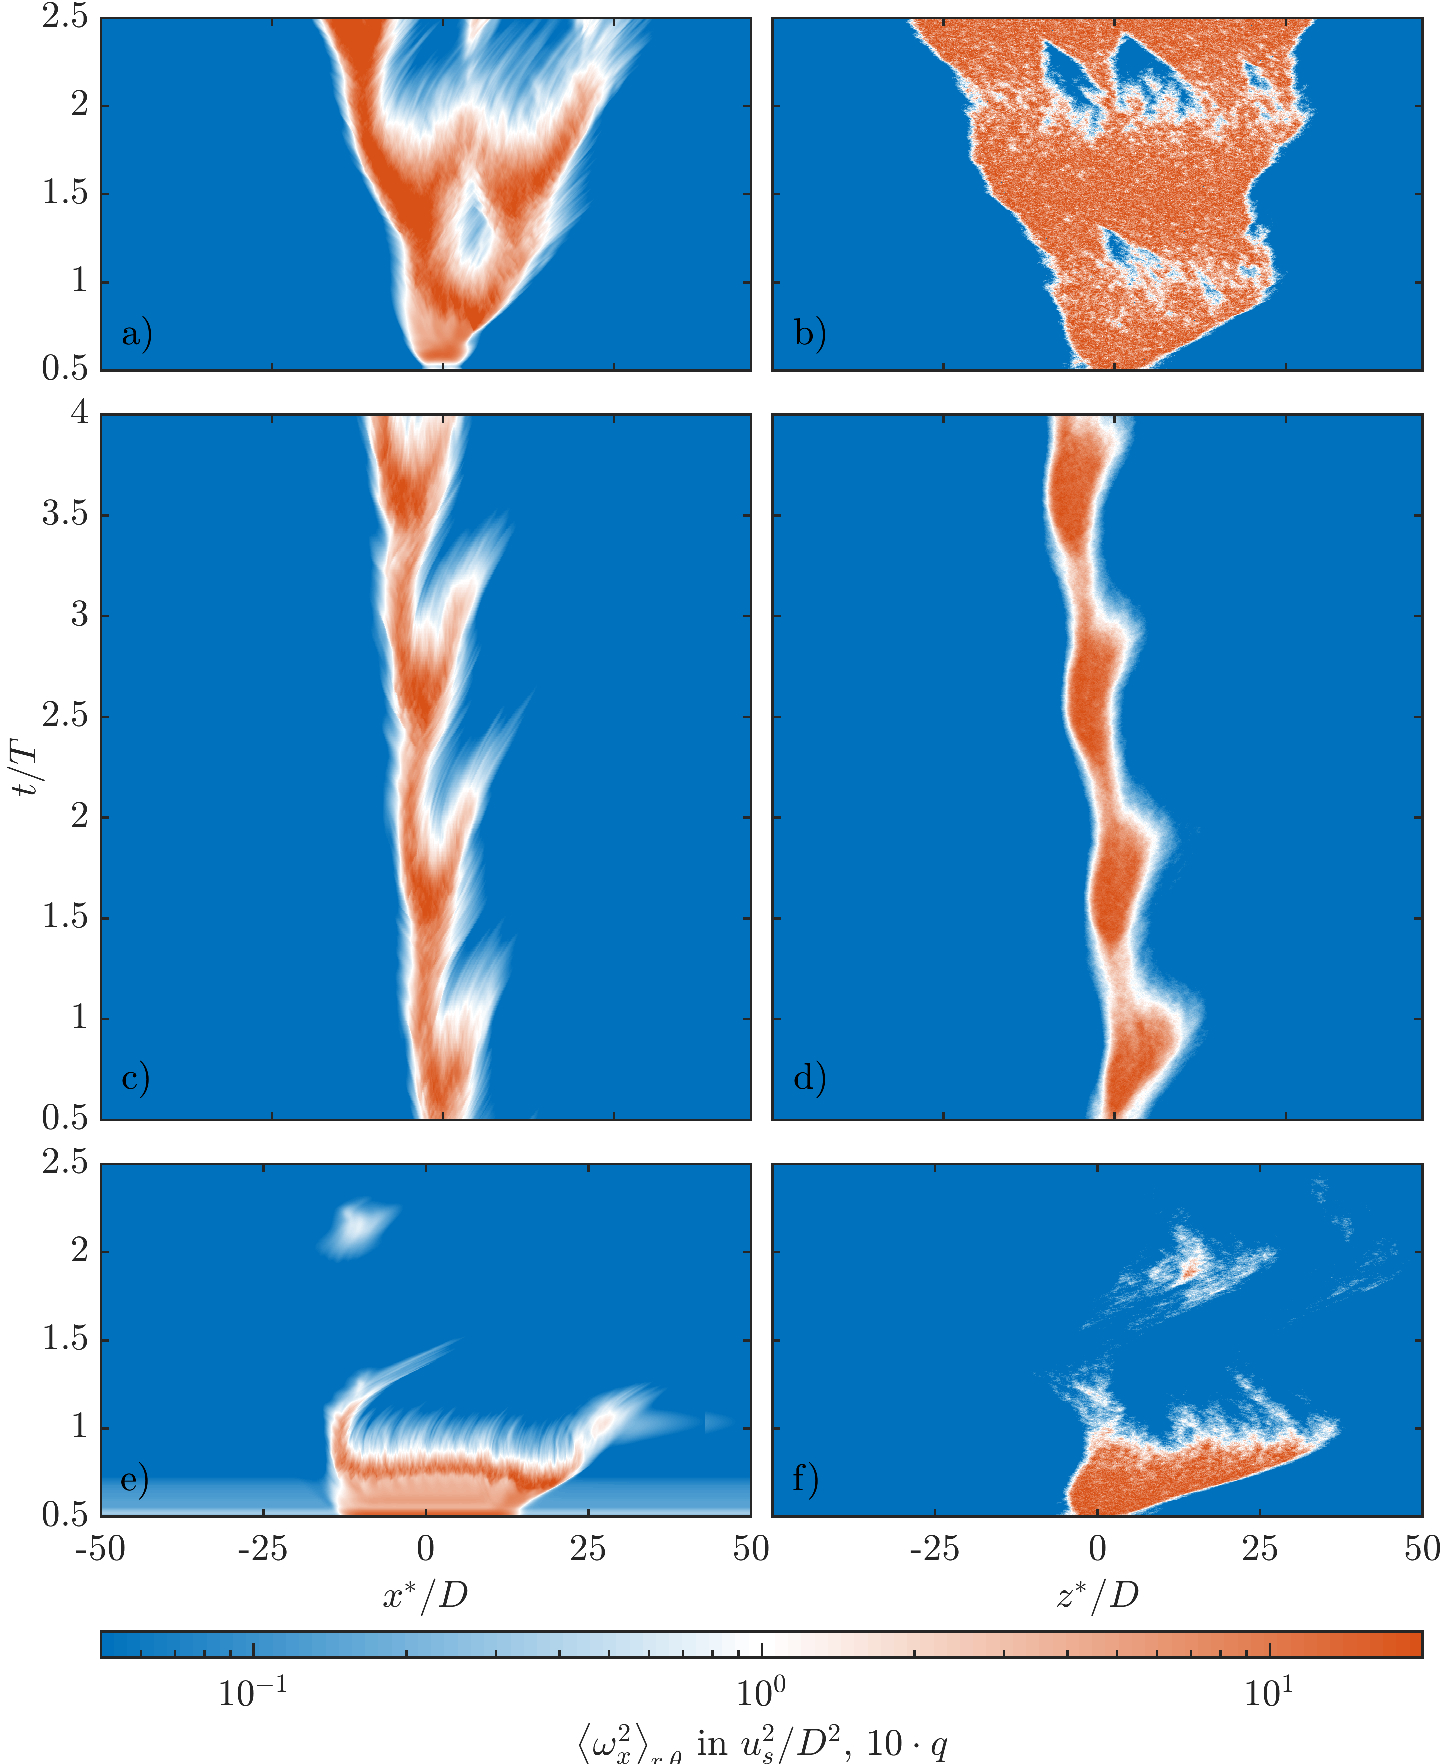
\includegraphics[width=\textwidth, trim=0mm 0mm 0mm 0mm, clip=true]{Figures9/Fig1.jpg}
\caption{Space-time diagram of the cross section integral of axial vorticity square (eq.~\eqref{eq:crosssc}) of DNS (left plots: a, c, e) and $10 \cdot q$ of the model (right plots b, d, f). The results correspond to DNS and model simulations in a $100D$ pipe. The DNS are initialised with the optimum perturbation scaled to $\left|\mathbf{u}^{\prime}_{0}\right|\approx 3e-2$ of magnitude and localized in a span of $5D$ following \cite{entropy2021}, while the model simulations with a localized puff of length $5D$. The figure is presented with respect to a moving frame $x^{*}$, moving with the bulk velocity $\bar{U}$. a) and b) correspond to $\Reynolds=3000$, $\Womersley=11$, $\Amplitude=0.5$. c) and d) correspond to $\Reynolds=2100$, $\Womersley=11$, $\Amplitude=0.75$. e) and f) correspond to $\Reynolds=2400$, $\Womersley=8$, $\Amplitude=1$. }
\label{fig:fig1}
\end{figure}
In figure~\ref{fig:fig1} we include three examples of DNS and model comparison, and in the appendix \dm{cita} comparisons for all the DNS in appendix~\dm{cita el correspondiente apendice con todas los parámetros de las DNS}. The model is able to capture reasonably well the turbulent front speed and turbulence survival in all the cases, as seen qualitatively in figure~\ref{fig:fig1} and the appendix. 






% - Phase average comparison of model and DNS...................................................................................
\subsection{Phase averaged puffs in pulsatile pipe flow}
In fig~\ref{fig:fig2}, we show a comparison between model simulations with $\sigma=0$ and phase averaged DNS results. At $\Reynolds=2100$, $\Womersley=11$ and $\Amplitude\leq 1$, turbulence is localized and modulated by the pulsation as in the case shown in fig.~\ref{fig:fig1}c) and d), see appendix \dm{Cita el apendice}. Although the model does not match perfectly the phase dependence and magnitude of $q^{*}$, see fig~\ref{fig:fig2}, both model and DNS show similar behaviours.

\begin{figure}
\centering
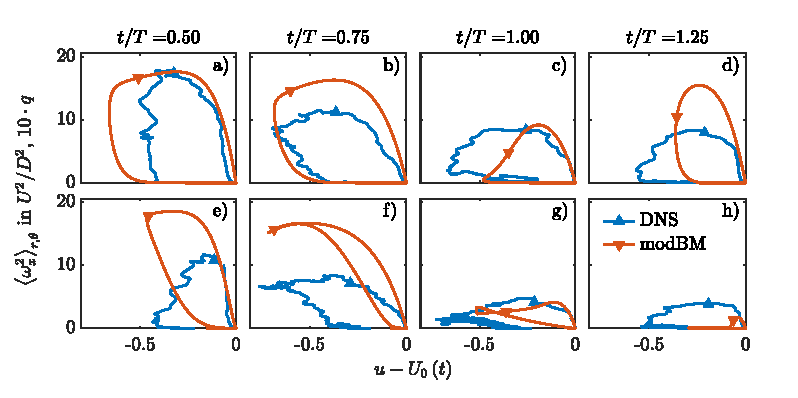
\includegraphics[width=\textwidth, trim=0mm 0mm 0mm 0mm, clip=true]{Figures9/Fig2.pdf}
\caption{Local phase space of turbulence indicator (axial vorticity in DNS and $10 \cdot q$ in model) and centerline velocity $u$ at different pulsation phases. The results correspond to phase averaged DNS for $30$ pulsation periods, and model simulations with $\sigma=0$ at $\Reynolds=2100$ and $\Womersley=11$. Cases a)-d) are for $\Amplitude=0.5$, cases e)-h) for $\Amplitude=1$. The phase of each subplot is indicated at the top of the corresponding subplot column.}
\label{fig:fig2}
\end{figure}

According to the local phase space in fig.~\ref{fig:fig2}a, b, e and f, the structures at $t/T\approx0.5$ and $t/T\approx0.75$ are similar to localized turbulent slugs, \cite{Song2017,barkley2016}, not to splitting puffs as was previously suggested by \cite{entropy2021}. According to the model at $\Amplitude=1$, fig.~\ref{fig:fig2}f, turbulence elongates into a strong slug, while at $\Amplitude=0.5$, fig.~\ref{fig:fig2}b, the structure is more similar to a weak slug. As $\bar{U}^{*}$ decreases at $t/T=1$, the magnitude $q^{*}$ of slugs also decreases, fig.~\ref{fig:fig2}c and g. At $t/T\approx 1.25$ the slug shrinks to its minimum length and magnitude, becoming a turbulent puff, fig.~\ref{fig:fig2}d and h. This modulation is similar for other cases, and depends on the exact combination of \Reynolds, \Womersley and \Amplitude.





% - Effect of ignoring new parameter...........................................................................................
\subsection{Effect of $\gamma$ and $\lambda$ in the EBM}
\begin{figure}
\centering
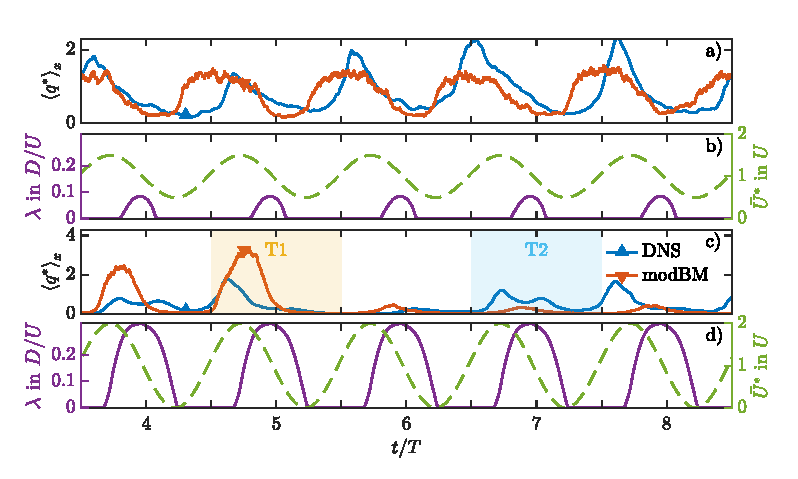
\includegraphics[width=\textwidth, trim=0mm 0mm 0mm 0mm, clip=true]{Figures9/Fig4.pdf}
\caption{a) and c): Volume integral of turbulence indicator $q^{*}$, with respect to time for two pulsatile pipe flows. b) and d): time evolution of $\bar{U}^{*}$ (dashed line) and $\lambda_{\max}$ phase shifted in time a quarter of the period. a) and c) correspond to $\Reynolds=2100$, $\Womersley=9$ and $\Amplitude=0.5$. b) and d) correspond to $\Reynolds=2100$, $\Womersley=9$ and $\Amplitude=1$. The shaded areas denote two periods of interest, where different turbulence behaviours are identified.}
\label{fig:fig4}
\end{figure}

In this section we explore the effects of including $\lambda$ in the model. As shown in fig~\ref{fig:fig3}, for the case of no instantaneous instability $\gamma=0$ the model behaves in two different ways. At $\Amplitude=0.5$, the results are almost identical to the case with $\gamma \geq 0$. At $\Amplitude \leq 0.5$ $\lambda$ is still quite small, fig~\ref{fig:fig4}b, and the dynamics are only dependant on the modulation due to the unsteady driving of the flow. At higher $\Amplitude=1$ however, puffs according to the model quickly decay for $\gamma=0$. This behaviour is not observed in DNS, where at $\Reynolds=2100$, $\Womersley=9$ and $\Amplitude=1$ puffs survive for several pulsation periods.

This would mean that turbulence in pulsatile pipe flow takes advantage of two mechanisms to survive. The first mechanism is the mean shear, that is maximum in the phases of the period where turbulence perceives $\bar{U}>U$. We propose that the second one is the instantaneous instability of the flow, that increases turbulence production during the phases when the laminar profile is instantaneously unstable. In our model the two mechanisms are represented by $r \cdot \textcolor{blue}{\bar{U}^{*}\left(t\right)}$ and $\textcolor{blue}{\gamma \cdot \lambda \left( t \right)}$ respectively.



% - Front speed and lifetimes using the model....................................................................................
\subsection{Parametric study using the EBM}
\begin{figure}
\centering
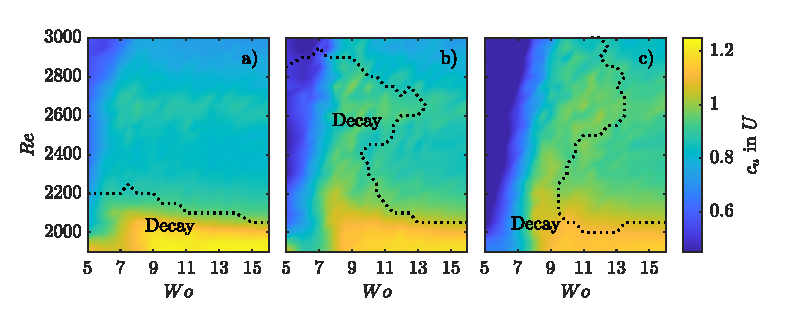
\includegraphics[width=\textwidth, trim=0mm 0mm 0mm 0mm, clip=true]{Figures9/Fig5.pdf}
\caption{Mean upstream front speed of $q$ according to simulations of the EBM at several \Reynolds and \Womersley for three different pulsation amplitudes. The results correspond to the interpolated front speed of $23\times20$ \Reynolds and \Womersley different combinations, for $N_{i}=10$ simulations each. In a) at $\Amplitude=0.5$, in b) at $\Amplitude=0.75$ in c) at $\Amplitude=1$. The dotted lines denote the threshold between \Reynolds and \Womersley cases where more than half of the $N_{i}$ simulations show turbulence decay $q\leq0.005$ before $t/T<5$.}
\label{fig:fig5}
\end{figure}

In this section use the model to perform simulations in a big \Womersley and \Reynolds parametric space for three different amplitudes. We consider $23$ equally spaced \Reynolds between $2050\leq \Reynolds \leq 3000$ and $20$ \Womersley between $5\leq \Womersley \leq 16$. For each combination of \Womersley, \Reynolds and \Amplitude we perform $N_{i}=10$ model simulations for $t/T<5$, and compute the mean upstream front speed of turbulence $c_{u}$. We stop the simulations at $t/T<5$, whenever turbulence decays in the whole domain, which we choose to correspond to $q \leq 0.005$, or when it fills the whole pipe. 

In figure~\ref{fig:fig5} we plot the upstream front speed $c_{u}$ together with our threshold for turbulence decay. The area distinguished by this threshold corresponds to cases where more than half of the $N_{i}$ simulations decay. The model does not perfectly reproduce the front speed and survival observed in DNS at certain \Reynolds, \Womersley and \Amplitude, but shows a similar behavior with respect to \Reynolds, \Womersley and \Amplitude.

At low amplitudes, $\Amplitude\leq0.5$ turbulence survival is mainly dependant on $\Reynolds$, fig.~\ref{fig:fig5}a. For $\Amplitude \geq 0.5$, the effect of the pulsation frequency becomes more important as $\Womersley$ decreases. In this regime the problem becomes more and more quasi-steady, and turbulence needs of a higher \Reynolds to survive as \Amplitude increases, as seen in figures~\ref{fig:fig5}b and c. For the \Womersley and \Amplitude we consider here, there is a sufficiently high \Reynolds at which turbulence is able to survive, fig.~\ref{fig:fig5}b. This critical \Reynolds increases as the amplitude \Amplitude increases.

Regarding the upstream front speed $c_{u}$, for all $\Amplitude$ but particularly at $\Amplitude \geq 0.75$, the front speed depends mainly on the size of the period in terms of advective time units $T=\frac{\pi \Reynolds}{2 \Womersley^{2}}$. As $T$ increases, either by increasing \Reynolds or decreasing \Womersley, the flow stays longer in phases of the period where turbulence elongates, $c_{u}<U$. This also means that turbulence stays longer in phases of the period where it tends to shrink and decay, $c_{u}>U$. However, the decay rate is faster than the elongation rate resulting in an average $c_{u}<U$. For sufficiently small $T$, as for $\Womersley \gtrsim 16$, the front speeds of steady pipe flow are recovered for all \Amplitude.




%%%%%%%%%%%%%%%%%%%%%%%%%%%%%%%%%%%%%%%%%%%%%%%%%%%%%%%%%%%%%%%
% SECTION: Limitiations of my model
\section{Limitations of the extended model}
When correctly fitted the EBM captures the dynamics of pulsatile pipe flow in a broad parametric regime, but it has some limitiations that need to be mentioned. In this section we comment on these limitations and also include some suggestions on possible ways to improve the model in future analysis. We differentiate between limitations that we understand are inherited from the original BM, and those that are new to the EBM.

As a general comment and different to the original BM, the EBM shows a much worse robustness with respect to the model parameters. Specially worrying are the dependence of the results to the noise intensity $\sigma$ and linear instability strength $\gamma$ parameters. 

In figure \dm{cita la figura}, we show the change in front speed when setting $\gamma$ or $\sigma$ constant. As observed in the figure the front speed, specially at high $\Amplitude>0.5$, diverges from the DNS results. 

\subsection{Limitations inherited from the BM}
The EBM is highly dependant on the parameter $\sigma$ and does not perfectly capture the shape of puffs and slugs as in the DNS case. We believe that these limitations are inherited from the original BM, as we describe below.

\subsubsection{The problem with parameter $\sigma$}
In the original BM, the paramater $\sigma$ was included in order to model puff decay, split and intermittency. As we explained in \dm{Cita el capitulo 5}, the original BM fails to capture the intermittent behaviour of localized turbulence in steady pipe flow at $2250 \lesssim \Reynolds \lesssim 2500$. In this regime, the model indicates that puffs elongate until they fill the whole domain with turbulence, while actual DNS show that in this regime turbulent patches (puffs or slugs) coexist with laminar patches. 

Coincidentally, for pulsatile pipe flow, at these $\Reynolds$ and $A>0.5$, according to our DNS \dm{aqui citare el futuro capitulo 7 donde espero enseñar todas las DNS que he calculado, y comentar mas a fondo el comportamiento de los puffetos} puffs remain localized for several $6\lessim Wo \lesssim 12$. If the parameter $\sigma$ is not scaled with $\Reynolds$, puffs at these flow parameters tend to elongate in the EBM. 

At lower $Re\approx 2100$, if $\sigma>0.5$ puffs in the EBM tend to decay much often that what they should, according to our DNS. Therefore, in order to capture the behaviour of puffs at these flow parameter, we must set $\sigma<0.5$. 

\subsubsection{The shape of elongated patches}
When one uses the EBM to study the shape of elongated turbulent structures at certain phases of the period, the model diverges from the DNS results. The EBM clearly overestimates the ratio between the magnitude of $q$ in the core of the turbulent patch and the magnitude of the upstream and downstream fronts. This was also observed in the case of slugs in the BM.


\subsubsection{The problems with parameter $\gamma$}
As described at the beginning of this chapter, the EBM was expected to work worse as $\Amplitude$ increases. At higher $\Amplitude$ the laminar profile becomes less similar to the simple parabolic profile of steady pipe flow \dm{cita el apendice con el catálogo de perfiles laminares}. In order to account for the shape of the pulsatile laminar profile, we proposed to use the instantaneous linear instability $\lambda$, and the parameter $\gamma$ that modulates it. Both work reasonably well, as long as $\gamma$ is correctly fitted. But as soon as $\gamma$ is changed puffs either decay or elongate when they shouldnot.

Also due to the definition of $\gamma$ the model overestimates the lifetime of puffs at certain flow parameters. In particular, according to the EBM, puffs at $10 \lesssim Wo \lesssim 15$, $A= 1$ and $1800 \lesssim \Reynolds \lesssim 2050$ survive the pulsation. This is obviously not observed in DNS of pulsatile pipe flow, where at $Re <2050$ and $A=1$ puffs tend to decay no matter the pulsation frequency. Moreover, at these flow parameters, the EBM are clearly dominated by the parameter $\lambda$, and therefore on $\gamma$. 

Our EBM considers that, as long as $\lambda>0$, turbulence can make use of the instantaneous linear instability to grow, but this may not be the case in a full DNS. At a given time step, the mean profile could be highly perturbed, and therefore be much different than the laminar profile. In this case, puffs would not have the chance to take advantage of the linear instability, and could even decay. This feature could be easily implented in the code by, setting $\gamma$ to zero at random periods during the integration.











% BIBLIOGRAPHY
\bibliographystyle{alpha}
\bibliography{sample}
\end{document}



% NEEDED MEDIA:
% - USING THE DNS the phase shift between qint/qmax y \bar{U}, a Re constante? Quizas Re=2100...
% - Grid convergence study of numerical method
% - Generate a (2 rows (Re) and 3 columns(A)) plot with the upstream front speed, with DNS results (when possible) and model results when not.  
% - Lifetimes at certain Re, Wo, and A

% NEEDED CITATIONS:
% Effect of pulsation Xu (2017?)
